% ============================================================================
% Paper 2 -- NeurReps 2026 extended abstract (4 pages excl. refs/appendix)
% Prose sections: Introduction, figures + captions, Related Work.
% Abstract and Conclusion were drafted separately; Results/Setup live in
% results_paper2.txt (generated by make_paper2_results.py) and the figures are
% generated by make_paper2_figs.py -- do not hand-edit numbers here without
% regenerating those.
%
% ALL NUMBERS BELOW ARE 3-SEED MEANS. Anything not traceable to
% results_paper2.txt or the two figure scripts must not appear in the paper.
% ============================================================================

\section{Introduction}

Continual learning with a pre-trained backbone is usually told as a story about
loss. A class is seen once, its prototype is recorded, and as the backbone
adapts to later tasks that prototype goes stale; accuracy on old classes falls,
and the fall is attributed to forgetting --- information about old classes being
overwritten. The remedies follow from the diagnosis: rehearse old data,
constrain the parameters, or freeze the backbone and give up on adaptation
altogether.

We begin from an observation that makes the diagnosis suspect. A prototype
read-out predicts $\arg\max_c \cos(\phi(x), \mu_c)$, and cosine similarity is
invariant under $O(d)$. So for any $R \in O(d)$ the pair
$(R\phi, \{R\mu_c\})$ induces \emph{exactly} the same classifier as
$(\phi, \{\mu_c\})$. The representation is therefore defined only up to a frame:
there is a gauge freedom, and the observable content of $\phi$ is the
frame-independent part. Adaptation is free to move the representation along that
gauge orbit without destroying anything --- but a \emph{stored} prototype does not
co-transform, so a read-out built before the motion will nonetheless fail after
it. That failure looks exactly like forgetting and is not.

Whether this matters is an empirical question about the map
$\Psi_t : \phi_0(x) \mapsto \phi_t(x)$ that adaptation induces. If $\Psi_t$ were
an element of $O(d)$, the accuracy drop would be pure bookkeeping, repaired
exactly by transporting $\mu_c \mapsto R_t \mu_c$. If $\Psi_t$ were an arbitrary
distortion, no such repair would exist and the forgetting story would be right.
We measure where between these poles real parameter-efficient adaptation falls.

We should be precise about the claim, because it is easy to overstate. This is
\emph{not} an exact symmetry of the trained network: adaptation genuinely changes
$\phi$, and nothing forces the change to be an isometry. What we claim, and
measure, is that the \emph{induced} change is approximately confined to a gauge
orbit, and that the observed forgetting is dominated by a read-out that fails to
co-transform rather than by a loss of class information.

Four measurements support this, on CIFAR-100 with a pre-trained ViT-B adapted by
shared LoRA, over a ten-task sequence, all as means over three seeds.

\textbf{The drift is affine.} Fitting a transport back to $\phi_0$ on held-out
old-class data, a learned MLP improves reconstruction cosine by $+0.004$ over a
linear map ($0.868 \to 0.868$) and is \emph{worse} in accuracy. Mapping back is
one matrix, not a kernel (Fig.~\ref{fig:affine}a).

\textbf{The drift is bounded and predominantly rotational.} The drift angle
saturates, $25.5^\circ \to 57.3^\circ$, rather than growing with depth, and a
single global rotation accounts for $80$--$83\%$ of it at every stage
(Fig.~\ref{fig:gauge}b).

\textbf{One rotation corrects it, at every depth.} A single orthogonal Procrustes
map applied to stale prototypes tracks a current-frame oracle to within
$0.40$ percentage points at \emph{all ten} stages, while uncorrected prototypes
decay by more than nine points (Fig.~\ref{fig:gauge}a).

\textbf{The residual is rotational again.} After the best linear transport, what
remains has preserved Gram structure ($0.964$) with $12.7^\circ$ of absolute
displacement --- the signature of an isometry --- and transported features retain
all class information ($73.9\%$ vs.\ $75.0\%$ for an oracle in its own frame).
The system is gauge-dominated at every scale we can resolve.

Taken together these say that the quantity adaptation should preserve is the
$O(d)$ invariant, not the absolute feature positions. That invariant is the Gram
matrix, and it yields a penalty that is flat along the gauge orbit and steep
orthogonal to it: it permits the harmless motion and forbids only non-rigid
distortion. Adding it raises the feature-quality ceiling from $74.9\%$ to
$81.6\%$, makes the drift measurably more rigid ($80.6\% \to 91.8\%$), and leaves
new-task accuracy untouched (Fig.~\ref{fig:affine}b). Representational forgetting,
measured as the gap between an oracle read-out and a frozen backbone, is
eliminated.

We also report where the account stops, because the limits are as informative as
the result. The repaired method only \emph{ties} a frozen read-out
($81.6\%$ vs.\ $81.5\%$): this backbone is near its ceiling on CIFAR-100 and
there is no adaptation headroom left to recover, so a win requires a benchmark
that has some. And the gauge reading explains prototype \emph{staleness} but not
representational \emph{degradation} --- without the penalty, the oracle itself
falls below frozen from the second task onward and the gap widens. Gauge
structure tells us what adaptation may safely change; it does not tell us where
changing it pays.

\paragraph{Contributions.}
\begin{enumerate}\itemsep0pt
  \item We identify the gauge freedom of a prototype read-out as the right frame
        for continual representation drift, and show empirically that
        PEFT-induced drift is approximately confined to that orbit: affine,
        bounded, $80$--$83\%$ rotational, and with a rotational residual.
  \item We show a single orthogonal Procrustes map recovers oracle accuracy at
        every depth of a ten-task sequence, so what is called prototype
        forgetting is largely a stale frame rather than lost content.
  \item We derive the intervention from the invariant rather than by search: a
        cosine-Gram penalty removes representational forgetting and, as a
        by-product, collapses seed variance from $\pm0.032$ to $\pm0.001$ ---
        what one expects if a degree of freedom is genuinely being removed.
  \item We state the ceiling: on a benchmark without adaptation headroom the
        repaired method ties a frozen read-out, and gauge structure does not
        address representational degradation.
\end{enumerate}

% ============================================================================
% FIGURES
% ============================================================================

\begin{figure}[t]
  \centering
  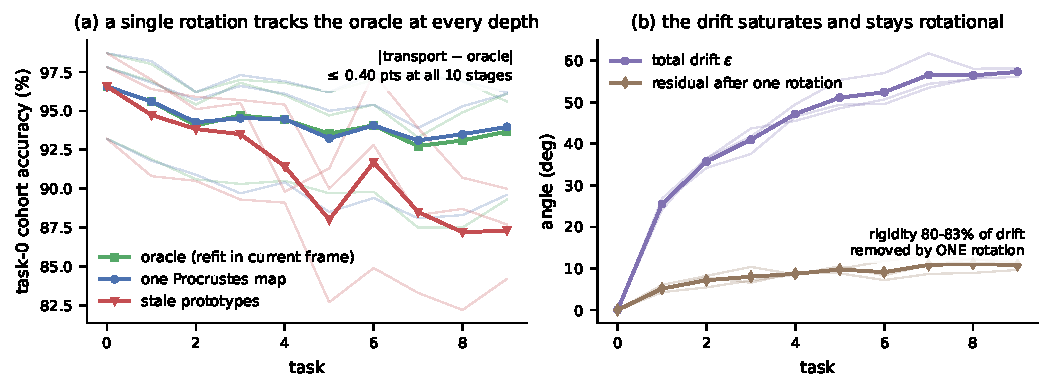
\includegraphics[width=\linewidth]{fig1_gauge.pdf}
  \caption{\textbf{The drift is a bounded, mostly-rotational gauge motion.}
    Task-0 cohort tracked through a ten-task sequence; thick lines are 3-seed
    means, thin traces individual seeds.
    \textbf{(a)} Uncorrected (\emph{stale}) prototypes decay by more than nine
    points, while a \emph{single} orthogonal Procrustes map fitted on the
    adapted features is indistinguishable from an \emph{oracle} that refits
    prototypes in the current frame --- the two agree to within $0.40$ percentage
    points at all ten stages. Prototype forgetting here is a change of frame, not
    a loss of content.
    \textbf{(b)} Total drift angle $\varepsilon$ \emph{saturates} near
    $57^\circ$ rather than accumulating, and the residual left after removing one
    global rotation stays small: $80$--$83\%$ of the drift is accounted for by a
    single rotation at every depth. The representation explores a bounded orbit.}
  \label{fig:gauge}
\end{figure}

\begin{figure}[t]
  \centering
  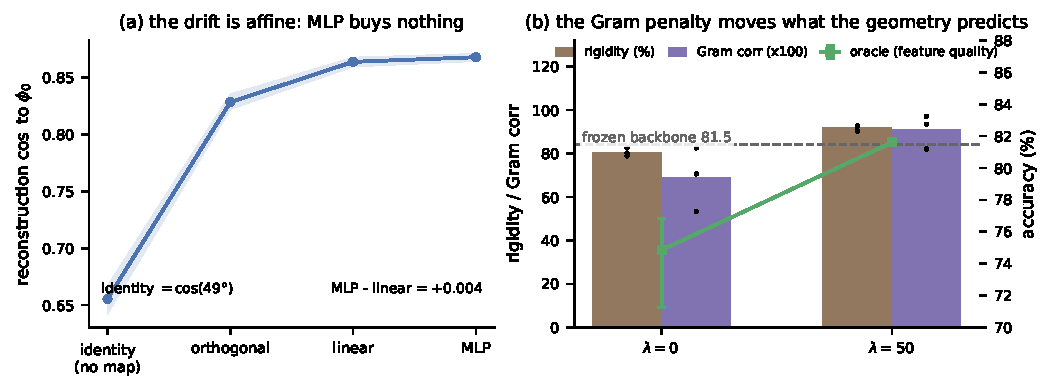
\includegraphics[width=\linewidth]{fig2_affine_gram.pdf}
  \caption{\textbf{The drift is affine, and the invariant prescribes the loss.}
    \textbf{(a)} Reconstruction cosine to $\phi_0$ for transports of increasing
    capacity, fitted on held-out old-class data. The curve saturates at
    \emph{linear}: an MLP adds $+0.004$ and is worse in accuracy, so the drift is
    affine at this measurement budget. The identity point,
    $\cos(49^\circ)$, independently reproduces the drift angle measured on a
    separate single-step protocol.
    \textbf{(b)} Adding a cosine-Gram penalty ($\lambda\!=\!0 \to 50$) moves
    exactly the quantities the gauge reading predicts: drift becomes more rigid
    ($80.6 \to 91.8\%$), Gram correlation rises ($0.69 \to 0.91$), and the
    feature-quality oracle crosses the frozen-backbone baseline
    ($74.9 \to 81.6$ vs.\ $81.5$). Dots are individual seeds. Because rotations
    leave the Gram matrix unchanged, the penalty is flat along the gauge orbit
    and steep orthogonal to it. Note the honest reading of the right axis: the
    repaired oracle \emph{ties} frozen rather than beating it.}
  \label{fig:affine}
\end{figure}

% ============================================================================
\section{Related Work}

\paragraph{Prototype drift in class-incremental learning.}
Semantic Drift Compensation~\citep{yu2020sdc} estimates the displacement of old
class prototypes from the drift of current-task data and corrects them by that
estimate; subsequent prototype-based continual learners inherit the same
treatment of drift as a nuisance displacement to be predicted. We differ in
kind rather than degree: we characterise the \emph{group structure} of the
displacement, show it is approximately an isometry, and therefore correct it with
one orthogonal map fitted once per stage rather than an estimated per-class
offset. The strong pre-trained-model baselines we measure against --- a frozen
backbone with a decorrelated random-feature head~\citep{mcdonnell2023ranpac} and
first-session-only adaptation~\citep{zhou2024revisiting} --- succeed precisely by
\emph{avoiding} drift, which is consistent with our finding that the harm lies in
a read-out that does not co-transform.

\paragraph{Symmetries of neural representations.}
That networks carry exact internal symmetries --- permutations of hidden units,
positive rescalings across ReLU layers --- is well
established~\citep{godfrey2022symmetries}, and exploiting them to align
\emph{independently trained} models underpins linear mode connectivity and
weight merging~\citep{entezari2022permutation,ainsworth2023rebasin}. Rotational
gauge freedom is likewise the reason representational-similarity analyses quotient
it out, whether by CKA~\citep{kornblith2019similarity} or by explicitly
Procrustes-based shape metrics~\citep{williams2021shape}, and the orthogonal
Procrustes solution itself is classical~\citep{schonemann1966procrustes}. Our
object of study is different: not the symmetry relating two separately trained
networks, but the orbit traced by a \emph{single} network as it adapts, and the
consequence of a downstream read-out that is invariant to that orbit while a
stored prototype is not.

\paragraph{Relational and Gram-based objectives.}
Distilling second-order structure rather than absolute activations is a
well-used technique: relational knowledge
distillation~\citep{park2019rkd} and similarity-preserving
distillation~\citep{tung2019similarity} both transfer pairwise structure and are
motivated by the intuition that ``structure'' transfers better than coordinates.
Our contribution here is not the loss but the \emph{argument} for it. In the
prototype-read-out setting the Gram matrix is not merely a convenient summary; it
is precisely the $O(d)$-quotient of the gauge freedom identified above, which is
why a Gram penalty is the correct shape --- flat along the harmless motion, steep
against the harmful one --- and why we can predict in advance which quantities it
should move.

\paragraph{Adaptation that damages transferable features.}
Our observation that adaptation can improve new-task accuracy while degrading
old-class features is consistent with evidence that fine-tuning distorts
pre-trained features and can underperform a linear probe out of
distribution~\citep{kumar2022lpft}. We add a decomposition of that damage: the
part that is a change of frame (large, and exactly repairable) and the part that
is genuine degradation (smaller, and untouched by any prototype geometry).

% ============================================================================
% NOTE on citations: keys above are placeholders to be checked against the
% actual bibliography before submission. Verify year, venue and author list for
% each -- particularly williams2021shape, godfrey2022symmetries and
% tung2019similarity, which are the ones I am least certain of.
% ============================================================================
